\documentclass[a4paper, 11pt]{article}

\usepackage[spanish]{babel}
\usepackage{amsmath}
\usepackage{titling}
\usepackage{graphicx}
\usepackage[colorinlistoftodos]{todonotes}
\usepackage{wrapfig}
\usepackage[utf8]{inputenc}
\begin{document}
\renewcommand{\contentsname}{Lista de Contenidos}
\renewcommand{\listfigurename}{Lista de Figuras}
\tableofcontents
\listoffigures
\thispagestyle{empty}
\newpage
\newcommand{\angstrom}{\mbox{\normalfont\AA}}
\begin{abstract}
En la siguiente practica se trató con cerámicos, se realizó un análisis XRD para comparar los gráficos obtenidos, pues al hacer una comparación de los picos de cada gráfica se puede inferir sobre cuales son los componentes principales de cada una de las muestras, adicionalmente se realizo un análisis gravimétrico para determinar que compuestos se evaporan y a que temperaturas, también se obtuvo gráficas para realizar su posterior análisis, las muestras otorgadas fueron de teja, cemento portland(geopolimero), ladrillo refractario y zeolita.
\end{abstract}
\section{Teor\'ia}
\setcounter{page}{1}
Los materiales cerámicos son compuestos químicos construidos por metales y no metales principalmente óxidos, nitruros y carburos, que incluyen minerales de arcillas, cementos y vidrios. Son minerales que son aislantes térmicos y que en medios de alta temperatura y corrosivos, son más resistentes que los metales y polímeros. Una las ventajas principales de los cerámicos es la alta dureza que tienen, pero también poseen una desventaja con respecto a la fragilidad que presentan.

Las cerámicas pueden presentar en forma vítrea, monocristalina, policristalina y combinaciones de algunas de ellas, donde la características de estos materiales es la capacidad de resistir al calor, y por otro lado la resistencia al ataque químico debida sustancialmente a la fortaleza de los enlaces entre sus átomos que les confiere un alto punto de fusión, dureza, y rigidez.
Los cerámicos son sólidos inorgánicos no metálicos producidos mediante tratamiento térmico. Comparados con los metales y plásticos son duros, no combustibles y no oxidables. Pueden utilizarse en ambientes con temperatura alta, corrosivos y tribológicos.
Una característica fundamental del cerámico incluye que puedan fabricarse en formas con dimensiones determinadas. Las propiedades de los materiales cerámicos cubren un amplio intervalo de necesidades, y son: mecánicas, térmicas, ópticas, eléctricas, magnéticas químicas.

\subsection{Procesado de Cerámicas}

El método más habitualmente empleado en la preparación de cerámicos consiste básicamente en dos etapas. El material de partida, polvo o partículas, es compactado en una matriz con la forma requerida, luego se procede a calentarla a elevadas temperaturas para conseguir que las partículas se enlacen entre si. Dependiendo del producto final requerido, en cuanto a propiedades, se realizan diferente variaciones al procedimiento como la adherencia de aglutinantes o lubricantes. Debe ser mezclado y el proceso puede ser llevado en seco o en húmedo. El medio de mezcla es el agua para la mayoría de los materiales preparados, aunque en casos particulares pueden usarse otros medios, como la cera en las cerámicas en alto contenido de alúmina. Para el conformado de los materiales normalmente se utilizan procesos generalmente en frío, como el prensado, el moldeo en bar-botina y la extrusión.\cite{cera}  

\subsubsection{Prensado}

Consiste en la compactación bajo presión de las materias primas pulverizadas, a las que normalmente se le añaden pequeñas cantidades de agua y pegamentos y lubricantes orgánicos. La mezcla adecuada de partículas de diferentes tamaños permite reducir al máximo los espacio intergranulares, en tanto que el medio húmedo facilita la distribución de las partículas disminuyendo el rozamiento. Además, y a diferencia de lo que ocurre en metalurgia en polvo, no se producen deformaciones plásticas en las partículas.   

Una vez conformado el material, es necesario someterlo a un tratamiento térmico que le dará la resistencia necesaria, es una parte fundamental del proceso, durante el mismo pueden aparecer importantes defectos como grietas, poros o distorsiones que obliguen a desechar la pieza producida. Los tratamientos térmicos normalmente incluyen dos etapas que son el secado y el cocido, y algunos materiales también se necesita el sinterizado.

\subsubsection{Secado}

Tiene como objetivo la eliminacion del agua o cualquier otra sustancia que se haya utilizado como aglutinante o lubricante. Normalmente la eliminacion de agua se hace a temperaturas inferiores a cien grados centigrados y se necesita menos de 24 horas. Para los aglutinante orgánicos es necesario llevar a cabo calentamientos a temperaturas de 200-300, e incluso mas en el caso que se tenga residuos de hidrocarburos. Durante el secado se produce una contracción en la pieza. La eliminación de moléculas de agua que rodean los granos provoca la disminución de la distancia entre partículas y la consiguiente contracción, es esta la razón por el cual, la velocidad de secado debe ser controlada. Las moléculas de agua se evaporan en la superficie del material. Por lo tanto el secado de la parte interna depende de la velocidad a la que esas moléculas difundan hasta la superficie. Si la velocidad de evaporación es mayor que la velocidad de difusión, la superficie externa se secara y contraerá antes que el interior, provocando la deformación dela pieza o su agrietamiento.

Despues del secado, el material cerámico, que en este estado se denomina cuerpo verde, es cocido.

\subsubsection{Cocido}


Para resolver los problemas que pudieran presentarse, tanto en la cocción de piezas desnudas como vidriadas, es importante conocer los fenómenos que ocurren durante la cocción.
Debe entenderse que dichos fenómenos suceden gradualmente a lo largo de un rango de temperaturas y algunos de ellos se solapan entre sí. 20 – 220 grados centigrados: periodo del vapor de agua; se evapora el agua de plasticidad y de los poros de la arcilla.
A menos que no haya agua física cuando se alcanzan los 100 grados centigrados, el punto de ebullición del agua, comenzará a formarse vapor de agua, que podría reventar la pieza si el proceso es demasiado rápido. Este proceso se debe desarrollar con suficiente lentitud para que toda el agua abandone la pieza sin causar ningún defecto. Para estar seguros, pueden calentarse las piezas durante ocho horas hasta llegar a 100. Si las piezas son de paredes delgadas y no especialmente delicadas podría bastar con menos tiempo, entre dos o tres horas podría ser suficiente. También debe tenerse en cuenta que cuanto más porosa sea la arcilla, más rápido se secará, o que un cacharro de pared excepcionalmente gruesa podría necesitar un precalentamiento de varios días. El clima también es un factor a tener en cuenta, por ejemplo, en lugares muy secos las piezas pueden contener muy poca agua cuando las metemos al horno y, en cambio, en zonas húmedas pueden tener una cantidad de agua tal que haga necesario un periodo más largo de precalentamiento.
220: comienza a descomponerse la materia vegetal contenida en la arcilla (lo cual produce olor), aunque esta no se quema completamente todavía. 
300 – 700: comienza a quemarse el carbón de la materia orgánica y se elimina el agua química.
Cualquier arcilla contiene cierta cantidad de materia orgánica que se quema durante la cocción. Si mirásemos dentro del horno en este rango de temperaturas, descubriríamos el carbón como pequeños puntos negros sobre las paredes de los cacharros, incluso en pastas de porcelana blanca.
450 - 600: el caolín se transforma en metacaolín y se elimina el agua química.
Este es el proceso, irreversible, por el que se forma la cerámica a partir de la arcilla. No solo hay agua física en la arcilla, sino también agua ligada químicamente que, igualmente, se elimina. Esta agua está asociada a la molécula de arcilla y una vez que se pierde, el material cambia para siempre. La arcilla se transforma en cerámica durante la cocción y el proceso no puede invertirse por ningún procedimiento sencillo.
  

\subsection{Difractómetro de rayos X}
Cuando los rayos X alcanzan un átomo interactúan con sus electrones exteriores. Estos reemiten la radiación electromagnética incidente en diferentes direcciones y con la misma frecuencia (en realidad debido a varios efectos hay pequeños cambios en su frecuencia). Este fenómeno se conoce como dispersión de Rayleigh (o dispersión elástica). Los rayos X reemitidos desde átomos cercanos interfieren entre sí constructiva o destructivamente. Este es el fenómeno de la difracción.\\

En el diagrama que sigue se esquematizan rayos X que inciden sobre un cristal. Los átomos superiores reemiten la radiación tras ser alcanzados por ella. Los puntos en los que la radiación se superpone constructivamente se muestran como la zona de intersección de los anillos. Se puede apreciar que existen ángulos privilegiados en los cuales la interferencia es constructiva, en este caso hacia la derecha con un ángulo en torno a 45º.

\subsection{Ley de Bragg}

La hipótesis de Bragg consiste en imaginar la difracción como una reflexión de los rayos X originada por "espejos" imaginarios formados por planos de átomos de la red cristalina (mostrados como lineas horizontales que pasan por los centros dispersores, es decir, por los átomos que se muestran como círculos azules en la imagen de la izquierda). Debido a la naturaleza repetitiva del cristal, estos planos estarían separados entre sí por distancias constantes d.\\
Los dos haces de rayos X, de longitud de onda $\lambda$, inciden en fase sobre sendos planos imaginarios, con un ángulo de incidencia $\theta$, y forman un frente de ondas (primera línea verde de la izquierda). \\
Para que exista reflexión cooperativa es necesario que tras la reflexión ambos haces sigan estando en fase (última linea verde de la derecha), situación que sólo ocurrirá si la diferencia de caminos recorridos  por los frentes de onda OF y OH (frentes de onda antes y después de la reflexión) es un número entero de veces la longitud de onda. 

\begin{figure}[h!] 
\centering
    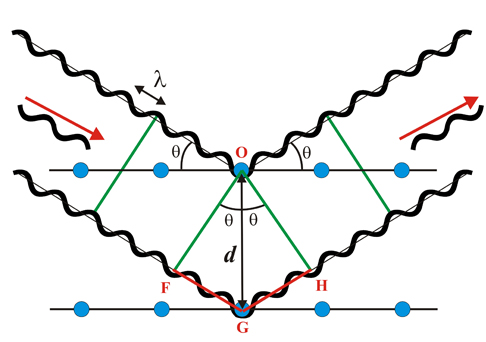
\includegraphics[scale=0.9]{bragg.png}
     \caption{Frentes de onda en fase}
    \label{ley_de_bragg1}
\end{figure}

Esa condición equivale a decir, que la suma de los segmentos FG y GH corresponde a un número entero (n) de veces la longitud de onda ($\lambda$):
$$FG+GH=n\lambda \;\;\;\;\;\;\;\;\; (1)$$ 

Tomando en cuanta que, $FG=GH$ y $sen(\theta)=\frac{FG}{d}$, al reemplazar en la ecuación 1 se tiene;

$$2dsin(\theta)=n\lambda \;\;\;\;\;\;\;\;\; (2)$$
Donde,
$n$ es un número entero,\\
$\lambda$ es la longitud de onda,\\
$d$ es la distancia entre los planos de la red cristalina y\\
$\theta$ es el ángulo entre los rayos incidentes y los planos de dispersión.\\
Todo lo citado anteriormente ocurre sólo cuando ambos frentes de onda se encuentra en fase como se observa en la Fig.\ref{ley_de_bragg1}, en caso de no suceder esto, no se cumple la Ley de Bragg Fig.\ref{ley_de_bragg2}.

\begin{figure}[h!] 
\centering
    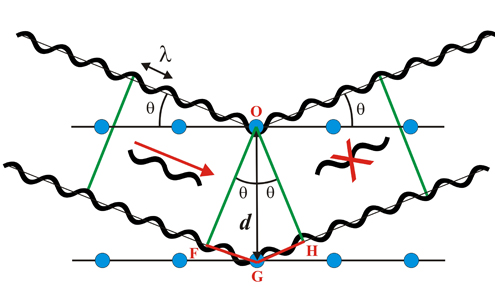
\includegraphics[scale=0.9]{bragg2.png}
     \caption{Frentes de onda desfasados}
    \label{ley_de_bragg2}
\end{figure}

Cuando la ley de Bragg tiene lugar debido a que los frentes de onda se encuentran en fase, se produce interferencia constructiva, por lo tanto la intensidad aumenta, en cambio cuando se encuentran desfasados se produce la interferencia destructiva, por consiguiente disminuye la intensidad \cite{no1}.



\section{Procedimiento Experimental}

Se realizó la práctica de Cerámicos con ayude tres diferentes muestras repartidas por el ingeniero. Cada grupo tomo una muestra en la que se debe obtener una pequeña porción para poder molerla en el crisol con ayuda del mortero, las muestras deben llegar al punto de quedar hechas casi polvo. Una vez hecho esto y dejando la estructura diminuta se lo lleva a los tamices que son una especie de cernidero, a diferencia que este posee medidas ya normalizadas. 
Un tamiz es el No. 325 de medida 45 um y el otro es el No. 400 de medida 38 um, la que nos ayudó para cernir  las muestras ya molidas y al final conseguir que la muestra sea más pura. Después de este proceso se necesita 1 gramo de cada material para poder colocarlo en el porta muestra y poder utilizarlo en el difractómetro de rayos x.  Que permite la identificación de estructuras cristalinas fundamentado en la ley de bragg. 
Para finalizar se lo lleva al termogravímetro (marca: TA, modelo: Q600, Serie: NNN.) en la que se mide el peso de una muestra frente al tiempo o a la temperatura mientras se somete la muestra a un programa de temperatura. En este obtendremos una gráfica conocida como termograma en la que se presenta el peso en el eje y versus la temperatura o tiempo en el eje x.


\section{An\'alisis de Resultados}

\subsection{XRD-X-Ray-Diffraction}

Por medio de la figura \ref{teja_xrd} se obtuvo las diferentes distancias interplanares utilizando la ley de bragg Ec. 2, el equipo ya nos otorgó las distancias más relevantes para el análisis. \\
Na-A se obtuvo $d=7.2\AA$, Ca-A $d=5\AA$.\\
En cuanto a la zeolita Fig.\ref{zeolita_xrd}, aproximadamente 35 minerales fue posible encontrar, entre estos;\\
La chabasita tiene una abertura elipsolidal con diámetro de $4.2 \AA$.\\
Analcima, es un mineral de clase silicato con formula química Na(Si2Al) con distancia interplanar $2.3129 \AA$\\
Clinoptilolita, mineral de clase tectosilicato con fórmula química (Ca,K,Na)\\6(Si30Al6) con distancia interplanar $5.352\AA$.\\
Erionita, mineral de clase tectosilicato con formula química (Ca,K,Na)\\n(Si26AL10) y distancia interplanar $11.745\AA$.\\
Mordenita, mineral tectosilicato con formula química (Na2,Ca,K2)4(Al8Si40) y distancia interplanar $14.612\AA$.
\\
\\
Para el cemento portland figura \ref{cemeportland_xrd} se obtuvo;\\
Portlandita con formula química CAH2O2 y sistema cristalino hexagonal que se encuentra entre las distancias interplanares de $3,5930\AA$ y $4,9090\AA$.\\
Ettingita, con formula química A12CA6H6 con sistema cristalino hexagonal que se encuentra entre las distancias interplanares de $11,2600\AA$ y $21,4800\AA$.\\
Calcite, con fórmula química CCAO3 con sistema cristalino romboidal que la podemos encontrar entre las distancias interplanares de $4,99\AA$ y $17,00\AA$.\\
Brownmillerita, con formula química ALCA2FEO5 y con sistema cristalino ortorrómbico que se encuentra entre las distnacias interplanares de $5,58\AA$ y $14,50\AA$.\\
Larnita, con formula química CA204SI y sistema cristalino monoclínico con distancias interplanares entre $5,51\AA$ y $9,32\AA$.\\
Hatrurita, con fórmula química CA305SI y sistema cristalino monoclínico que se encuentra entre las distancias interplanares de $7,07\AA$ y $12,23\AA$.\\
\\
Para el ladrillo refractario Fig. \ref{ladrillo_xrd} se obtuvo lo siguiente;\\
Cuarzo, es un mineral oxido con compuesto químico SiO2 con distancia interplanar de $3.34\AA$.\\
Calcita, es un mineral carbonato con compuesto químico CACO3 y con distancia iunterplanar de $3.03\AA$.\\
Dolomita, es un mineral compuesto de carbonato de calcio y magnesio con compuesto químico CaMg(CO3)2 y con distancia interplanar de $2.88\AA$.\\
Feldespastos, mineral aluminisicato con compuesto químico (K,Na,Ca,Ba,NH4)(Si,Al)4O8   y distancia interplanar de $3.24\AA$.\\



\subsection{TGA-Termogravimétrico}
\
\\
Teja Fig.\ref{teja_tga}, se obtuvo lo siguiente;\\
\\
A $70.83^{\circ}C$ se tiene un 4\% de peso, a $154.77^{\circ}C$ se tiene un 75\% de peso, a $657.28^{\circ}C$ se tiene 81\% de peso, a $822.82^{\circ}C$ se tiene 73\% de peso, y a $921.13^{\circ}C$ se tiene 70\% de peso.
\\
\\
Zeolita Fig.\ref{zeolita_tga}, se obtuvo lo siguiente;\\
\\
A $41,71^{\circ}C$ tendremos un 98.6\% de peso, a los $106.55^{\circ}C$, se tiene 94.5\% de peso, a los $182.82^{\circ}C$ se tiene 93.8\% de peso, a los $311.22^{\circ}C$ se tiene 92.8\% de peso, a los $801.92^{\circ}C$ se tiene 92.5\% de peso y a los $883.28^{\circ}C$ se tiene 92\% del peso.
\\
\\
Cemento Portland Fig.\ref{cemeportland_xrd}, se obtuvo lo siguiente;\\
\\
A $88,18^{\circ}C$ tendremos un 95\% de peso, a los $129.80^{\circ}C$, se tiene 100.5\% de peso, a los $399.73^{\circ}C$ se tiene 94.5\% de peso, a los $668^{\circ}C$ se tiene 98\% de peso, a los $865^{\circ}C$ se tiene 95\% de peso.
\\
\\
Ladrillo refractario Fig.\ref{ladrillo_tga}, se obtuvo lo siguiente;\\
\\
A $56.33^{\circ}C$ se tiene un 97\% de peso, a $667,81^{\circ}C$ se tiene un 97.5\% de peso, a $706.16^{\circ}C$ se obtuvo 97.8\% de peso, a $782.85^{\circ}$ se tiene 96.9\% de peso, a $835.32^{\circ}C$ se tiene 96.3\% de peso.


\section{Conclusiones}

Al hacer una comparación de las temperaturas y el porcentaje de peso Fig. \ref{comparacion} se obtuvo que el ladrillo refractario es el que menos se evapora, es decir, perde menor cantidad de masa al aumentar la temperatura, esta es una de las razones por la que este ladrillo es ampliamente usado para los hornos de fundición ya que soportan altas temperaturas, y no se desea que el horno se funda a alguna temperatura de operación, siendo esta un ventaja muy favorable para estas condiciones de uso, seguidamente se obtuvo que la teja, la zeolita y el cemento portland, este ultimo disminuye de forma mas notoria debido a que la presencia de agua también es mayor en comparación al resto de materiales.

Los cerámicos cambian sus propiedades acorde a su composición química y a la temperatura en que se hayan sinterizado las mismas.
Al obtener un producto final, este a ser expuesto a elevadas temperaturas, dependiendo de su composición química, empieza a degradarse, perdiendo un porcentaje de masa, lo que cambiaría sus propiedades, tanto físicas como químicas.


\begin{thebibliography}{9}

\bibitem{cera}
José L. Mesa, Materiales Cerámicos, (1990), Universidad del País Vasco, Departamento de Química Inorgánica, Disponible en: http://joseluismesarueda.com/documents/TEMA\_7\_001.pdf, Fecha de Consulta: 15/08/2016

\bibitem{no1}
Department of Crystallography and Structural Biology, Deducción e interpretación informal de la Ley de Bragg, (2016), Disponible en: http://www.xtal.iqfr.csic.es/Cristalografia/parte\_05\_5.html, Fecha de Consulta: 15/08/2016

\bibitem{no2}
Escuela Superior Politécnica del Litoral, Área de Materiales, Guía de Laboratorio de Materiales de Ingeniería, Práctica 4- Cerámicos, I-Término,(2016)

\bibitem{no3}

W.D. Kingery, H.K. Bowen, D.R. Uhlmann, Introduction to Ceramics, Second Edition, (1976), John Wiley, USA, New York

\end{thebibliography}
\newpage      

\section{Anexos}

\begin{figure}[h!] 
\centering
    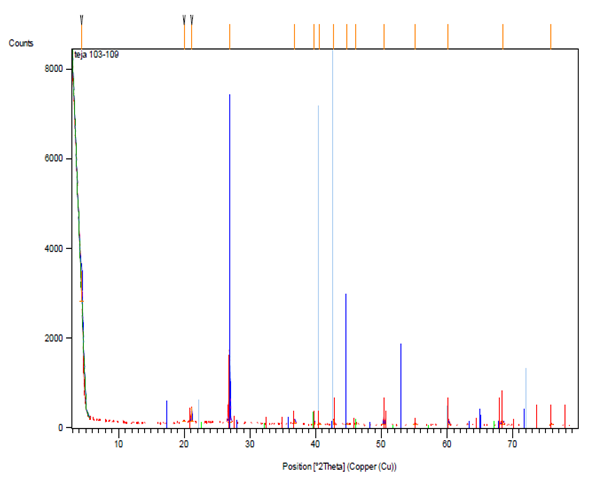
\includegraphics[scale=0.6]{teja1.png}
     \caption{XRD Teja}
    \label{teja_xrd}
\end{figure}

\begin{figure}[h!] 
\centering
    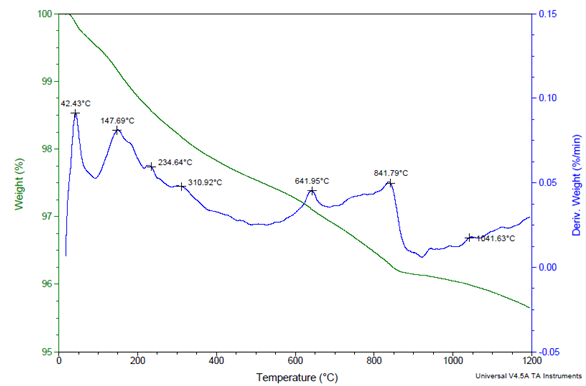
\includegraphics[scale=0.7]{teja2.png}
     \caption{TGA Teja}
    \label{teja_tga}
\end{figure}

\begin{figure}[h!] 
\centering
    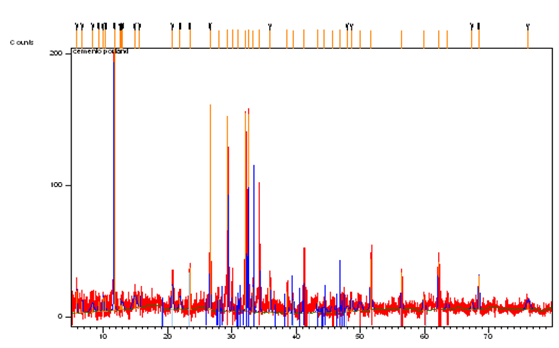
\includegraphics[scale=0.9]{zeolita1.png}
     \caption{XRD Zeolita}
    \label{zeolita_xrd}
\end{figure}

\begin{figure}[h!] 
\centering
    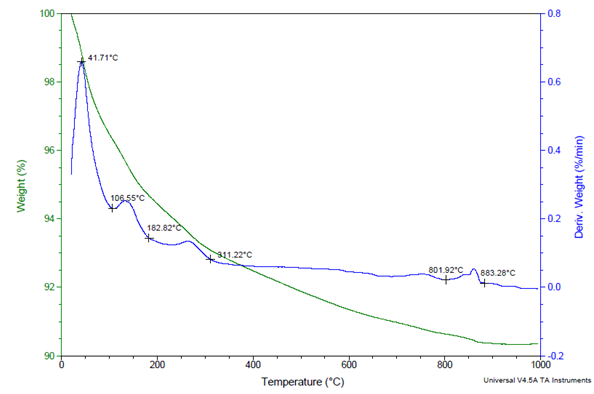
\includegraphics[scale=0.9]{zeolita2.png}
     \caption{TGA Zeolita}
    \label{zeolita_tga}
\end{figure}

\begin{figure}[h!] 
\centering
    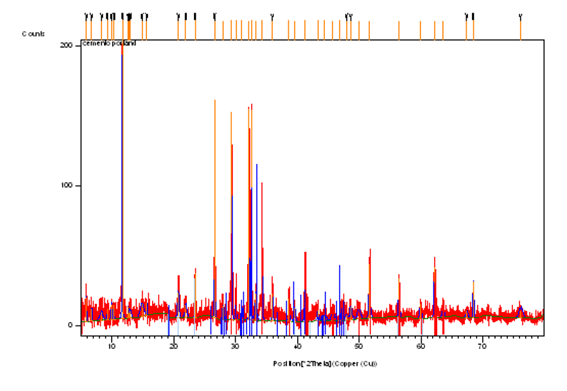
\includegraphics[scale=0.9]{cemeportland2.png}
     \caption{XRD Cemento Portland (Geopolimero)}
    \label{cemeportland_xrd}
\end{figure}

\begin{figure}[h!] 
\centering
    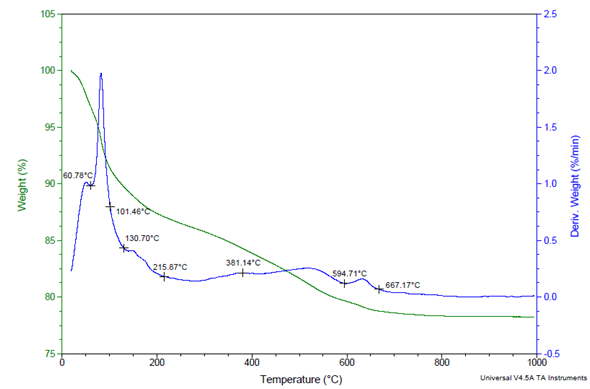
\includegraphics[scale=0.9]{cemeportland3.png}
     \caption{TGA Cemento Portland (Geopolimero)}
    \label{cemeportland_tga}
\end{figure}

\begin{figure}[h!] 
\centering
    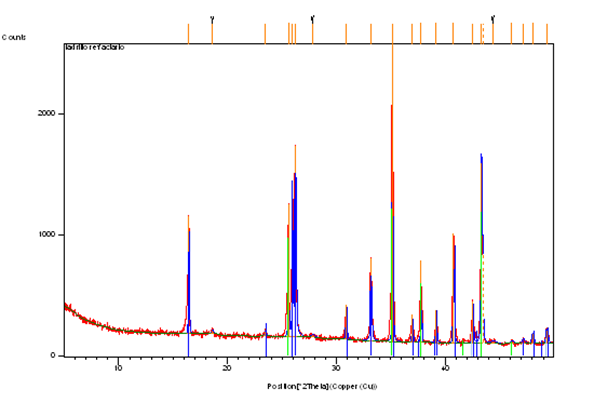
\includegraphics[scale=0.9]{ladrillo1.png}
     \caption{XRD Ladrillo Refractario}
    \label{ladrillo_xrd}
\end{figure}


\begin{figure}[h!] 
\centering
    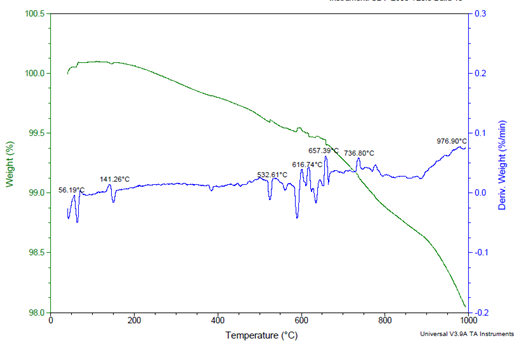
\includegraphics[scale=0.9]{ladrillo2.png}
     \caption{TGA Ladrillo Refractario}
    \label{ladrillo_tga}
\end{figure}


\begin{figure}[h!] 

    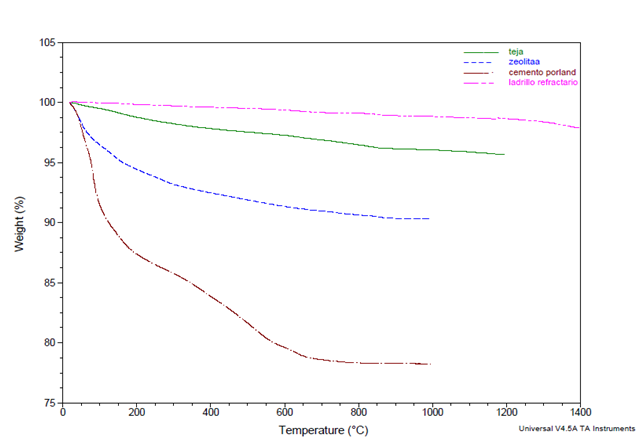
\includegraphics[scale=0.75]{comparacion.png}
     \caption{Comparación}
    \label{comparacion}
\end{figure}

\end{document}    